\section{Theoretical and Conceptual Framework}
\label{sec:theoreticalframework}

\begin{figure}[h] % h stands for 'here'
    \centering
    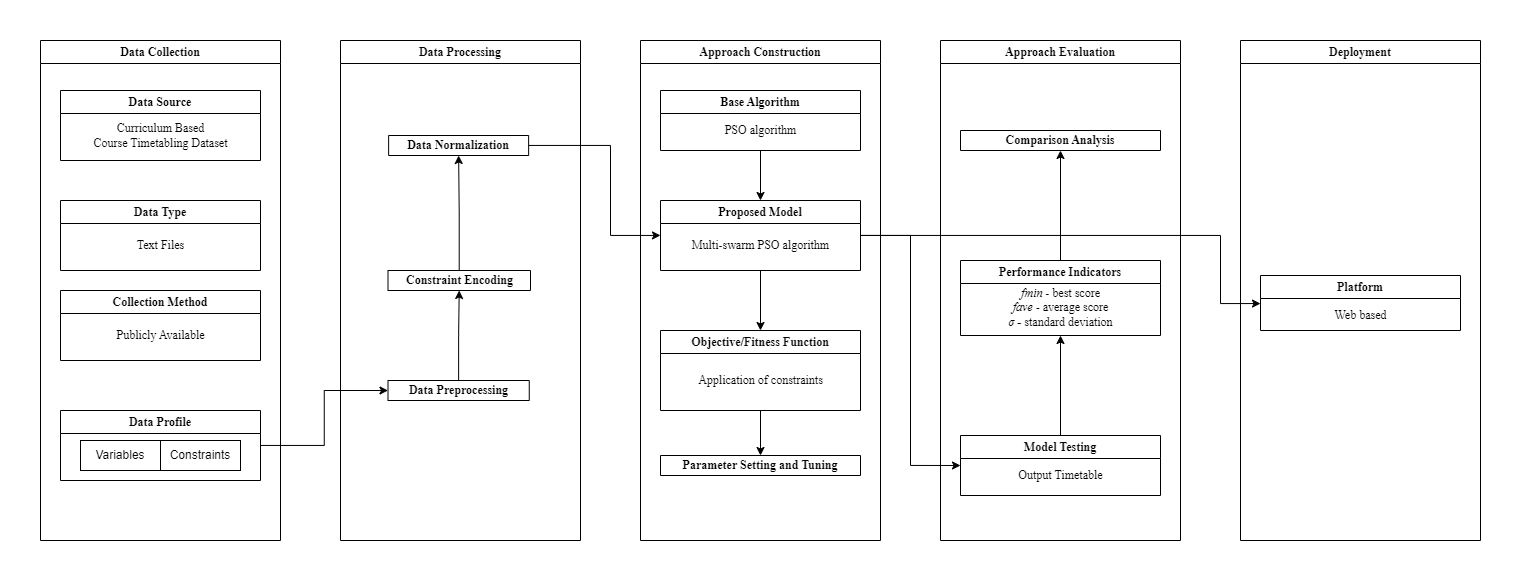
\includegraphics[width=1\textwidth]{framework}
    \caption{Theoretical and Conceptual Framework}
    \label{fig:framework} % label for referencing
\end{figure}

The theoretical and conceptual framework of this study consists of five separate yet connected components: Data Collection, Data Processing, Approach Construction, Approach Evaluation, and Deployment. The workflow starts with the Data Collection phase, collecting benchmark datasets and optimization problem instances. These datasets usually are publicly available and typically represented in text or XML formats. This phase ensures that there is adequate sourcing and data variety to support the solid analysis of the optimization model against different conditions. Steps undertaken in the Data Processing step include cleaning the data to remove inconsistencies and make sure that all inconsistencies in constraints are encoded in apt forms of mathematics for solving before preparing the data for optimized use. Data cleaning removes errors or missing values that could have otherwise affected the model's performance while encoding constraints take problem-specific rules and transform them into a format that could be used by the model. Normalization and data categorization are also considered uniform since the optimization model can cope well with the data. All these processes, therefore, collectively provide standardized and reliable input for the optimization phase. This ensures that the information is valid and appropriate to the model in question. It will act as a foundation for later phases.

The construction of the approach deals with the creation of the model of multi-swarm optimization. This acts as a core method for the optimization problem solution. A part of this component deals with the base model setup and setting parameters that make the model capable of appropriately addressing the needs of the problem. The Approach Evaluation phase involves testing the performance of the model based on whether it satisfies any required objectives. This phase must be done to determine how well the proposed model is and make adjustments according to what is needed to increase its applicability. Lastly, the solution would be deployed by presenting an optimized solution via the use of a web-based interface, where users will have the ability to upload their problem instances and find real-time optimized outputs for their respective problems. All parts are included to be effective contributors to the solution development process, ensuring that data is handled properly, models built and evaluated appropriately, and the final solution is practically deployable. 

\subsection{Concepts, Theories, and Methodologies Reused}

This paper employs current swarm intelligence theories and algorithms, mainly in Particle Swarm Optimization (PSO) \cite{kennedy1995particle} and Multi-Swarm Optimization (MSO) \cite{MultiSwarm2004} \cite{Blackwell2006-ms}. PSO is an established algorithm to efficiently search large solution spaces by a set of particles that are exploring a search area with individual and collective experiences. Parsopoulos and Vrahatis \cite{parsopoulos2002recent} first introduced neighborhood-based swarming in global and local variants in the introduction of the MSO approach. That paper set a solid basis for multi-swarm frameworks. The structure of the neighborhood and dynamic tuning of parameters discussed there provided important inspirations for later developments in multi-swarm optimization. One of the first spectacular applications of these multi-swarm approaches is given by Blackwell and Branke \cite{MultiSwarm2004}, who studied MSO in dynamic settings. These methodologies are crucial to establish the foundation for MPSO.

\subsection{Concepts, Theories, and Methodologies Modified}

To improve existing PSO and MSO methodologies, the research here modifies the base methodologies to take on a multi-swarm structure particularly designed for UCTP, called MPSO. The MPSO algorithm divides the main swarm into smaller, specialized sub-swarms operating in parallel to explore the solution space more effectively at different parts. \cite{XIA2018126} \cite{MultiSwarm2004} \cite{Blackwell2006-ms} The improvement is designed to circumvent the limitations of lack of search diversity and trapping into local optima through the encouragement of a greater exploration of solution possibilities along with the exploitation of promising regions. The modification improves better adaptability and efficiency in generating feasible course timetables.

\subsection{Novel Concepts, Theories, and Methodologies Introduced}

This research introduces a new optimization approach for UCTP via MPSO, specifically designed to address complex timetabling constraints such as room availability, faculty preferences, and scheduling conflicts. Its novelty lies in the combination of dynamic swarm partitioning and targeted exploration, allowing the MPSO algorithm to achieve workload balance and enhance resource use within educational institutions \cite{Bacanin2022-multiswarm}. The proposed MPSO-based methodology balances mechanisms for exploration and exploitation, ensuring that the different solution domains are discovered thoroughly to allow the provision of optimal scheduling solutions.